\documentclass[sigconf]{acmart}

\usepackage{booktabs} % For formal tables
\usepackage{amssymb}
\usepackage{mathtools}
\usepackage{multirow}
\usepackage{listings}
\usepackage{indentfirst}
\usepackage{verbatim}
\usepackage{amsmath, amssymb}
\usepackage{graphicx}
\usepackage{xcolor}
\usepackage{url}
\usepackage{stmaryrd}
\usepackage{xspace}
\usepackage{comment}
\usepackage{wrapfig}
\usepackage[caption=false]{subfig}
\usepackage{placeins}
\usepackage{tabularx}
\usepackage{ragged2e}

\def\transarrow{\xrightarrow}
\newcommand{\setarrow}[1]{\def\transarrow{#1}}

\newcommand{\trule}[2]{\frac{#1}{#2}}
\newcommand{\crule}[3]{\frac{#1}{#2},\;{#3}}
\newcommand{\withenv}[2]{{#1}\vdash{#2}}
\newcommand{\trans}[3]{{#1}\transarrow{#2}{#3}}
\newcommand{\ctrans}[4]{{#1}\transarrow{#2}{#3},\;{#4}}
\newcommand{\llang}[1]{\mbox{\lstinline[mathescape]|#1|}}
\newcommand{\pair}[2]{\inbr{{#1}\mid{#2}}}
\newcommand{\inbr}[1]{\left<{#1}\right>}
\newcommand{\highlight}[1]{\color{red}{#1}}
\newcommand{\ruleno}[1]{\eqno[\scriptsize\textsc{#1}]}
\newcommand{\rulename}[1]{\textsc{#1}}
\newcommand{\inmath}[1]{\mbox{$#1$}}
\newcommand{\lfp}[1]{fix_{#1}}
\newcommand{\gfp}[1]{Fix_{#1}}
\newcommand{\vsep}{\vspace{-2mm}}
\newcommand{\supp}[1]{\scriptsize{#1}}
\renewcommand{\G}{\mathfrak G}
\newcommand{\sembr}[1]{\llbracket{#1}\rrbracket}
\newcommand{\cd}[1]{\texttt{#1}}
\newcommand{\miniKanren}{miniKanren\xspace}
\newcommand{\ocanren}{OCanren\xspace}
\newcommand{\free}[1]{\boxed{#1}}
\newcommand{\binds}{\;\mapsto\;}
\newcommand{\dbi}[1]{\mbox{\bf{#1}}}
\newcommand{\sv}[1]{\mbox{\textbf{#1}}}
\newcommand{\bnd}[2]{{#1}\mkern-9mu\binds\mkern-9mu{#2}}

\newcommand{\meta}[1]{{\mathcal{#1}}}
\renewcommand{\emptyset}{\varnothing}

\lstdefinelanguage{ocanren}{
keywords={fresh, let, in, match, with, when, class, type,
object, method, of, rec, repeat, until, while, not, do, done, as, val, inherit,
new, module, sig, deriving, datatype, struct, if, then, else, open, private, virtual, include, success, failure,
true, false},
sensitive=true,
commentstyle=\small\itshape\ttfamily,
keywordstyle=\ttfamily\underbar,
identifierstyle=\ttfamily,
basewidth={0.5em,0.5em},
columns=fixed,
fontadjust=true,
literate={fun}{{$\lambda$}}1 {->}{{$\to$}}3 {===}{{$\equiv$}}1 {=/=}{{$\not\equiv$}}1 {|>}{{$\triangleright$}}3 {\\/}{{$\vee$}}2 {/\\}{{$\wedge$}}2 {^}{{$\uparrow$}}1,
morecomment=[s]{(*}{*)}
}

\lstset{
mathescape=true,
basicstyle=\small,
identifierstyle=\ttfamily,
keywordstyle=\bfseries,
commentstyle=\scriptsize\rmfamily,
basewidth={0.5em,0.5em},
fontadjust=true,
language=ocanren
}

\usepackage{letltxmacro}
\newcommand*{\SavedLstInline}{}
\LetLtxMacro\SavedLstInline\lstinline
\DeclareRobustCommand*{\lstinline}{%
  \ifmmode
    \let\SavedBGroup\bgroup
    \def\bgroup{%
      \let\bgroup\SavedBGroup
      \hbox\bgroup
    }%
  \fi
  \SavedLstInline
}
%\addtolength{\parskip}{-2pt}
\pagestyle{plain}


% Copyright
%\setcopyright{none}
%\setcopyright{acmcopyright}
%\setcopyright{acmlicensed}
\setcopyright{rightsretained}
%\setcopyright{usgov}
%\setcopyright{usgovmixed}
%\setcopyright{cagov}
%\setcopyright{cagovmixed}


% DOI
%\acmDOI{10.475/123_4}

% ISBN
%\acmISBN{123-4567-24-567/08/06}

%Conference
%\acmConference[WOODSTOCK'97]{ACM Woodstock conference}{July 1997}{El
%  Paso, Texas USA}
%\acmYear{1997}
%\copyrightyear{2016}


%\acmArticle{4}
%\acmPrice{15.00}

% These commands are optional
%\acmBooktitle{Transactions of the ACM Woodstock conference}
%\editor{Jennifer B. Sartor}
%\editor{Theo D'Hondt}
%\editor{Wolfgang De Meuter}

\begin{comment}
First, the evaluation needs to give more information. How many cases did you try, and where can we download those specifications? Substantiate your claims of comparable or faster performance using quantitative data. What are some cases where the improvement almost works but unfortunately fails? Why restrict your claims to "the queries which return a finite number of answers"?

Second, the improvement should be described using the formal framework already set up in Section 2. That would clarify the description towards the end of Section 4. As it stands, it is not completely clear what "a greedy approach" is -- given the knowledge that "the list of conjuncts diverges", the question remains as to how to reorder the conjuncts and sometimes go "even more back" (as mentioned in Section 5.1). In other words, the paper should show and explain what Figure 2 becomes with the improvement. Only then is the claim of "quadratic time" meaningful.

Chapter 4 continues the discussion on the problem of non-commutativity of conjunctions and proposes the optimization technique progressively. But the completed version of the optimization algorithm is not clearly stated in an individual paragraph. At least a short summary on the core algorithm of this paper should be necessary. A more detailed and formal one would even be better.

The paper talks about the effectiveness of the optimization, however, a reader may be interested in the limitation of this technique. Since the divergence test is sufficient but not necessary, the paper may discuss about when this optimization works and when it does not.

My main problem with this paper is its presentation. Much of the paper
is devoted to a formal system of syntax and semantics. I find the
description there long winded, and does not highlight the non-standard
parts if there is any. To make the matter worse, the formal system is
not used at all, as no result is presented in the main text. Even if
space is an issue, at least the main theorem shall be presented.

I also find the section of implementation and evaluation slightly
disappointing. No detail of the deep embedding is shown, and the a few
examples are by no means an “evaluation”. I am also confused by the
very informal nature of the presentation in this section. For example,
how is the problem with “perm” solved? Since the problem is that the
evaluation goes both directions, how can reordering help? I also do
not understand the example of Binary arithmetic as very little code is
shown.
\end{comment}

\sloppy

\begin{document}

\title{Improving Refutational Completeness\\
of Relational Search via Divergence Test}

\titlenote{Produces the permission block, and
  copyright information}

\author{Dmitri Rozplokhas}
\affiliation{%
  \institution{St. Petersburg Academic University}
  \streetaddress{Khlopina st., 8-3-А}
  \city{St. Petersburg}
  \state{Russia}
  \postcode{194021}
}
\email{rozplokhas@gmail.com}

\author{Dmitri Boulytchev}
\affiliation{%
  \institution{St. Petersburg State University}
  \streetaddress{Universitetskaya emb., 7-9}
  \city{St. Petersburg}
  \state{Russia}
  \postcode{199034}
}
\email{dboulytchev@math.spbu.ru}

% The default list of authors is too long for headers.
%\renewcommand{\shortauthors}{B. Trovato et al.}

\begin{abstract}
We describe a search optimization technique for implementation of relational programming language
miniKanren which makes more queries to converge. Our technique is based on a certain 
divergence criterion, which we use to trigger a dynamic reordering of subgoals. We present a formal semantics of
miniKanren-like language, and prove, that our optimization does not compromise already
converging programs, thus being a proper improvement. We also present the prototype
implementation of improved search and demonstrate its application for a number of
useful specifications.
\end{abstract}

%
% The code below should be generated by the tool at
% http://dl.acm.org/ccs.cfm
% Please copy and paste the code instead of the example below.
%
\begin{CCSXML}
<ccs2012>
<concept>
<concept_id>10003752.10003790.10003795</concept_id>
<concept_desc>Theory of computation~Constraint and logic programming</concept_desc>
<concept_significance>500</concept_significance>
</concept>
<concept>
<concept_id>10003752.10010124.10010131.10010134</concept_id>
<concept_desc>Theory of computation~Operational semantics</concept_desc>
<concept_significance>100</concept_significance>
</concept>
<concept>
<concept_id>10011007.10011006.10011008.10011009.10011015</concept_id>
<concept_desc>Software and its engineering~Constraint and logic languages</concept_desc>
<concept_significance>500</concept_significance>
</concept>
</ccs2012>
\end{CCSXML}

\ccsdesc[500]{Theory of computation~Constraint and logic programming}
\ccsdesc[100]{Theory of computation~Operational semantics}
\ccsdesc[500]{Software and its engineering~Constraint and logic languages}

\keywords{relational programming, refutational completeness, divergence test}

\maketitle

\section{Introduction}

Relational programming is an approach, based on the idea of describing programs not as functions, but 
as relations, without distinguishing between the arguments and the result value. This technique makes it 
possible to ``query'' programs in various ways, for example, to execute them ``backwards'', finding
all sets of arguments for a given result. Relational behavior can be reproduced using a number of
logic programming languages, such as Prolog, Mercury~\cite{Mercury}, 
or Curry~\cite{Curry}. 
There is also a family of embedded DSLs, specifically designed for writing declarative relational
programs that originates from \miniKanren~\cite{TRS}. \miniKanren is a minimalistic 
declarative language, initially developed for Scheme/Racket. The smallest implementation of \miniKanren 
is reported to comprise of only 40 LOC~\cite{MicroKanren,2016}; there are also more elaborate versions, including
\miniKanren with constraints~\cite{CKanren,CKanren1}, user-assisted search~\cite{Guided}, nominal unification~\cite{AlphaKanren},
etc. Due to its simplicity, \miniKanren was implemented for more than 50 other languages, such as
Haskell, Go, Smalltalk, and OCaml. In a nutshell, miniKanren introduces a minimalistic set of constructs to describe
relations over a set of syntactic terms, thus providing the same expressivity as a pure core of conventional
logic programming\footnote{A detailed miniKanren to Prolog comparison can be found at \url{http://minikanren.org/minikanren-and-prolog.html}}. 

\miniKanren has proven to be a useful tool to provide elegant solutions for various problems, otherwise considered as
non-trivial~\cite{WillThesis}. One of the most promising areas of application for \miniKanren is the implementation of
\emph{relational interpreters}. Such interpreters are capable not only to interpret programs in various directions, but also
to infer programs on the basis of expected input-output specification~\cite{Untagged}.

Being quite simple and easy to use by design, in implementation \miniKanren introduces some subtleties. Under the hood, \miniKanren 
uses a complete interleaving search~\cite{Search}. This search is guaranteed to find all existing solutions; however, it can diverge, when no 
solution exists. In reality, this amounts to divergence in a number of important cases~--- for example, when a program is asked to 
return \emph{all} existing solutions, or when the number of requested solutions exceeds the number of existing ones.
It is often possible to refactor the specification of a concrete query to avoid the divergence, but this has to be done for every execution
``direction'' of interest that compromises the idea of fully declarative relational programming.

The specifications that do not diverge even when no solutions exist, are called \emph{refutationally complete}~\cite{WillThesis}. Writing 
refutationally complete relational specifications nowadays requires knowledge of \miniKanren implementation intrinsics, and is not always
possible due to the undecidability of the fundamental computability problems. However, by developing a more advanced search it is possible
to make more specifications refutationally complete.

In this work we address one particular problem that often leads to refutational incompleteness~--- the non-commutativity of
conjunction. We present an optimization technique that is based on a certain non-termination test. Our optimization
is \emph{online} (performed during the search), \emph{non-intrusive} (does not introduce new constructs and does not require
any changes to be made to the existing specifications), and \emph{conservative} (applied only when the divergence
is detected). We prove that for the queries that return a finite number of answers, our optimization preserves convergence. 
We also demonstrate the application of the optimization for a number of interesting and important problems.

We express our gratitude to William Byrd and the reviwers of this paper for their constructive remarks and suggestions.


\section{The Source Language and Relational Extension}

In this section we present a formal description of a small functional language, taken as a source
for relational conversion. We describe its syntax, typing rules and semantics, and then extend it
with relational constructs. Thus, relational conversion maps a program in the source language into 
the program in extended. We specify the typing rules and semantics for the extension as well.

\subsection{The Source Language}
\label{source_language}

The syntax of our source functional language is shown on Figure~\ref{functional_syntax}. It consists of a lambda calculus, 
enriched with constructors with fixed arities $C^n$, patterns $p$ and pattern-matching constructs. Among constructors
we distinguish two nullary interpreted constructors \lstinline|true| and \lstinline|false|, and we add a boolean equality
operator ``$=$'' and expressions for recursive/non recursive let-bindings. In a pattern matching we only allow shallow
patterns (which is not an essential limitation) and do not allow wildcards (which is important~--- converting 
wildcard pattern matching into relational form would require essentially different projections). This choice of language may 
look quite a restrictive. However, in terms of relational programming the language contains virtually everything we would need. Indeed, from
relational conversion standpoint the standard built-in integer arithmetics, for example, is of no use~--- 
there is simply no way to convert integer expression into relational form, using integer expressions. In order to use relational 
arithmetics one needs to reimplement everything from scratch, using, for example, Peano encoding; but Peano arithmetics can be
easily expressed in the language we present.

\begin{wrapfigure}{r}{0.5\textwidth}
\centering
%\scalebox{0.9}{
$$
\begin{array}{rcl}
   e &=&x\\
     & &\lambda x.e\\
     & &e_1\;e_2\\
     & &C^n(e_1,\dots, e_n)\\
     & &\lstinline|true|\\
     & &\lstinline|false|\\
     & &\lstinline|let $x$ = $e_1$ in $e_2$|\\
     & &\lstinline|let rec $f$ = $\lambda x.e_1$ in $e_2$|\\
     & &e_1\,=\,e_2\\
     & &\lstinline|match $e$ with $\{p_i$ -> $e_i\}$|\\
     & &\\
   p &=&C^n(x_1,\dots,x_n)\\
\end{array}
$$
%}
\caption{The syntax of the source language}
\label{functional_syntax}
\end{wrapfigure}

Our language is equipped with Hidley-Milner type system, and we present the typing rules in conventional syntax-directed form 
on Figure~\ref{functional_typing}. Besides primitive boolean type, type variables and function types our system contains
a number of implicitly defined algebraic datatypes $T^k$, and we stipulate, that each constructor $C^n$ belongs to exactly one
datatype. In rule \textsc{Constr$_T$} we assume, that type $t^C$ has the form $T^k(t_1,\dots,t_k)$, where each of the types
$t_i$ is recovered from the types $t_i^C$ of arguments of constructor $C^n$ and, moreover, these types are agree in the sense of
constructor application. Similarly, in rule \textsc{Match$_T$} the types of all $C_i^{k_i}(x^i_1,\dots,x^i_{k_i})$ are expected
to be equal $t^C$, and $t^{C_i}_j$ is a type of $j$-th argument of constructor $C_i$, used in a pattern.

\setarrow{:}
\newcommand{\typed}[3]{\withenv{#1}{\trans{#2}{}{#3}}}

\begin{figure}
\centering
{\bf Types:}
$$
\begin{array}{rcll}
  \mathcal X &=&\alpha, \beta, \dots                                            &\mbox{\supp{(type variables)}}\\
  \mathcal D &=&T^n,...                                                         &\mbox{\supp{(datatype constructors)}}\\
  \mathcal T &=&\lstinline|bool|\mid\alpha\mid T^k(t_1,\dots,t_k)\mid t_1\to t_2 &\mbox{\supp{(types)}}\\
  \mathcal S &=&\forall\bar{\alpha}.t                                           &\mbox{\supp{(type schemas)}}
\end{array}
$$
{\bf Typing rules:}
\def\arraystretch{0}
\begin{tabular}{p{7cm}p{7cm}}
$$
\typed{\Gamma}{\lstinline|true|,\;\lstinline|false|}{\lstinline|bool|}
\ruleno{Bool$_T$}
$$ 
&
$$
\trule{\typed{\Gamma}{e_1}{t}\;\;\;\;\typed{\Gamma}{e_2}{t}}
      {\typed{\Gamma}{e_1=e_2}{\lstinline|bool|}}
\ruleno{Eq$_T$}
$$
\\
$$
\trule{\typed{\Gamma}{e_i}{t^C_i}}
      {\typed{\Gamma}{C^n(e_1,\dots,e_n)}{t^C}}
\ruleno{Constr$_T$}
$$
&
$$
\typed{\Gamma,x:\forall\bar{\alpha}.t}{x}{t[\bar{\alpha}\gets\bar{t^\prime}]}
\ruleno{Var$_T$}
$$
\\
$$
\trule{\typed{\Gamma}{f}{t_1\to t_2}\;\;\;\;\typed{\Gamma}{e}{t_1}}
      {\typed{\Gamma}{f\;e}{t_2}}
\ruleno{App$_T$}
$$
&
$$
\trule{\typed{\Gamma,\,x:t_1}{f}{t_2}}
      {\typed{\Gamma}{\lambda x.f}{t_1\to t_2}}
\ruleno{Abs$_T$}
$$
\\
\multicolumn{2}{p{14cm}}{
$$
\trule{\typed{\Gamma}{e_1}{t_1}\;\;\;\;\typed{\Gamma,x:\forall\bar{\alpha}.t_1}{e_2}{t}}
      {\typed{\Gamma}{\lstinline|let $\;x\;$ = $\;e_1\;$ in $\;e_2$|}{t}},\;\bar{\alpha}=FV(t_1)\setminus FV(\Gamma)
\ruleno{Let$_T$}
$$}\\
\multicolumn{2}{p{14cm}}{
$$
\trule{\typed{\Gamma,f:t_1}{\lambda x.e_1}{t_1}\;\;\;\;\typed{\Gamma,f:\forall\bar{\alpha}.t_1}{e_2}{t}}
      {\typed{\Gamma}{\lstinline|let rec $\;f\;$ = $\;\lambda x.e_1\;$ in $\;e_2$|}{t}},\;\bar{\alpha}=FV(t_1)\setminus FV(\Gamma)
\ruleno{LetRec$_T$}
$$}\\
\multicolumn{2}{p{14cm}}{
$$
\trule{\typed{\Gamma}{e}{t^C}\;\;\;\;\typed{\Gamma,x^i_1:t^{C_i}_1,\dots,x^i_{k_i}:t^{C_i}_{k_i}}{e_i}{t}}
      {\typed{\Gamma}{\lstinline|match $\;e\;$ with $\;\{C_i^{k_i}(x^i_1,\dots,x^i_{k_i})$ -> $e_i\}$|}{t}}
\ruleno{Match$_T$}
$$}
\end{tabular}
\caption{Typing rules for the source language}
\label{functional_typing}
\end{figure}

We describe the semantics of our language in the form of transition system. The transition relation

\setarrow{\to}
\newcommand{\step}[2]{\trans{\inbr{#1}}{}{\inbr{#2}}}

$$
\step{\mathcal S,\,e}{\mathcal S^\prime,\,e^\prime}
$$

\noindent describes one step of evaluation of expression $e$ with a stack of contexts $\mathcal S$, which results in
a new stack $\mathcal S^\prime$ and a new expression $e^\prime$. A context is an expression with a unique hole; informally speaking, 
a stack of contexts describes a path in the expression being evaluated from the topmost construct to the point, where the evaluation 
currently is taking place. For a context $C$ and an expression $e$ we denote by $C[e]$ a complete expression with no holes, which is 
obtained by plugging $e$ into the unique hole of $C$. From each state $\inbr{C_1:C_2:\dots:C_k,e}$ we can build an 
expression $C_k[\dots[C_2[C_1[e]]\dots]$, which represents an intermediate result of evaluation according to a small-step semantics. 
This form of semantic description originates from Felleisen-style~\cite{Felleisen} approach for small-step semantics, and we've
chosen it since it can be naturally extended for relational case.

Our semantics describes call-by-value left-to-right evaluation; in the rules $\textsc{Beta}$, $\textsc{Mu}$, $\textsc{LetVal}$,
$\textsc{LetRec}$ and $\textsc{MatchVal}$ we perform capture-avoiding substitutions, which respect the names in abstractions and let-bindings,
and in the rules $\textsc{EqTrue}$ and  $\textsc{EqFalse}$ we assume, that values being compared do not contain subvalues of the 
form $\lambda x.e$ or $\mu f\lambda x.e$. Finally, in the rule $\textsc{MatchVal}$ we assume, that at most one pattern matches the 
scrutinee~--- this is an important distinction with usual semantics of pattern matching, when the patterns are examined in a top-down 
manner until the match succeeds.

Finally, for a closed expression $e$ and a value $v$ we write $\sembr{e}=v$, iff 

$$\inbr{\epsilon,e}\to^*\inbr{\epsilon,v}$$

\noindent where $\epsilon$~--- an empty stack, and ``$\to^*$'' is a reflexive-transitive closure of ``$\to$''.

\begin{figure}[t]
\centering
{\bf Values:}
$$
\mathcal V = \lstinline|true|\mid\lstinline|false|\mid C^n(v_1,\dots,v_n)\mid\lambda x.e\mid\mu f\lambda x.e
$$
{\bf Contexts:}
$$
\mathcal C = \Box\;e\mid v\;\Box\mid\lstinline|let $x$ = $\Box$ in $e$|\mid\lstinline|match $\;\Box\;$ with $\{p_i$->$e_i\}$|\mid C^n(\bar{v},\Box,\bar{e})\mid\Box=e\mid v=\Box 
$$
$$
C[e]\mbox{\supp{~--- a context $C$ with an expression $e$ plugged into a hole}}
$$
{\bf Stack of contexts:}
$$
\mathcal S=\epsilon\mid\mathcal C : \mathcal S
$$
{\bf States:}
$$
\inbr{\mathcal S, e}\mbox{\supp{(stack of contexts, expression)}};\;\inbr{\epsilon,e}\mbox{\supp{(initial state)}};\;\inbr{\epsilon,v}\mbox{\supp{(final state)}}
$$
{\bf Transitions:}
\vskip2mm
\bgroup
\def\arraystretch{0}
\begin{tabular}{p{7cm}p{7cm}}
\multicolumn{2}{p{14cm}}{
$$
\step{C:\mathcal S,\, v}{\mathcal S,\, C[v]}\ruleno{Value}
$$}\\
$$
\step{\mathcal S,\, f\;e}{\Box\;e:\mathcal S,\, f}\ruleno{AppL}
$$&
$$
\step{\mathcal S,\, v\;e_2}{v\;\Box:\mathcal S,\, e_2}\ruleno{AppR}
$$\\
$$
\step{\mathcal S,\,e_1=e_2}{\Box=e_2:\mathcal S,\,e_1}\ruleno{EqL}
$$&
$$
\step{\mathcal S,\,v=e}{v=\Box:\mathcal S,\,e}\ruleno{EqR}
$$\\
\multicolumn{2}{p{14cm}}{
$$
\step{C:\mathcal S,\,v=v}{\mathcal S,\,C[\lstinline|true|]}\ruleno{EqTrue}
$$}\\
\multicolumn{2}{p{14cm}}{
$$
\step{C:\mathcal S,\,v_1=v_2}{\mathcal S,\,C[\lstinline|false|]},\;v_1\ne v_2\ruleno{EqFalse}
$$}\\
\multicolumn{2}{p{14cm}}{
$$
\step{\mathcal S,\, (\lambda x.e)\;v}{\mathcal S,\, e[x\gets v]}\ruleno{Beta}
$$}\\
\multicolumn{2}{p{14cm}}{
$$
\step{\mathcal S,\, (\mu f\lambda x.e)\;v}{\mathcal S,\, e[f\gets\mu f\lambda x.e,\, x\gets v]}\ruleno{Mu}
$$}\\
\multicolumn{2}{p{14cm}}{
$$
\step{\mathcal S,\, C^n(v_1,\dots,v_{k-1},e_k,\dots,e_n)}{C^n(v_1,\dots,v_{k-1},\Box,\dots,e_n):\mathcal S,\, e_k}\ruleno{Constr}
$$}\\
\multicolumn{2}{p{14cm}}{
$$
\step{\mathcal S,\, \lstinline|let $\;x\;$ = $\;e_1\;$ in $\;e_2$|}{\lstinline|let $\;x\;$ = $\;\Box\;$ in $\;e_2$|:\mathcal S,\, e_1}\ruleno{Let}
$$}\\
\multicolumn{2}{p{14cm}}{
$$
\step{\mathcal S,\, \lstinline|let $\;x\;$ = $\;v\;$ in $\;e$|}{\mathcal S,\,e[x\gets v]}\ruleno{LetVal}
$$}\\
\multicolumn{2}{p{14cm}}{
$$
\step{\mathcal S,\, \lstinline|let rec $\;f\;$ = $\;\lambda x.e_1\;$ in $\;e_2$|}{\mathcal S,\, e_2[f\gets\mu f\lambda x.e_1]}\ruleno{LetRec}
$$}\\
\multicolumn{2}{p{14cm}}{
$$
\step{\mathcal S,\,\lstinline|match $\;e\;$ with $\;\{p_i$->$e_i\}$|}{\lstinline|match $\;\Box\;$ with $\;\{p_i$->$e_i\}$|:\mathcal S,\, e}\ruleno{Match}
$$}\\
\multicolumn{2}{p{14cm}}{
$$
\step{\mathcal S,\,\lstinline|match $\;C_k^{n_k}(v_1,\dots,v_{n_k})\;$ with $\;\{C_i^{n_i}(x^i_1,\dots,x^i_{n_i})\to e_i\}$|}{\mathcal S,\,e_k[x^k_j\gets v_j]}\ruleno{MatchVal}
$$}
\end{tabular}
\egroup
\caption{Semantics for the source language}
\label{functional_semantics}
\end{figure}

\FloatBarrier

\subsection{Relational Extension}
\label{relational_extension}

The relational extension adds five conventional miniKanren expressions for constructing goals; the syntax is shown on Figure~\ref{relational_syntax}.
Since relational constructs are added to regular functional ones, it becomes possible to construct expressions like \lstinline|fun x.x = (true === fun y.y)| etc.
In order to rule such pathological expressions out we devised an extension for the type system of source language. In fact, this approach follows the
actual implementation for OCaml, where a careful choice of types for representing terms and goals made it possible to reject the majority of non-well-formed
programs at compile-time.

Our extension for the type system introduces one interpreted datatype constructor $\Box^o$ with one data constructor $\uparrow$~--- a polymorphic type and
a constructor for logical terms. In addition we introduce interpreted type of goals $\G$, which is distinct from all other types. The typing rules for the relational 
extension are shown on Figure~\ref{relational_typing}. These rules describe rather expected typing: in unification and disequality constraints only
terms of the same logical type can be used, and conjuction and disjunction can only be taken for goals. Note, in our extension a term can be calculated as
a result of arbitrary expression in initial functional language (as long as this expression has expected logical type), but such ``higher-order'' terms will
never appear as a result of relational conversion, so, in fact, relational extension we describe here defines a richer language, than we actually need.

\begin{wrapfigure}{r}{0.5\textwidth}
\centering
$$
\begin{array}{rl}
   e\mathrel{{+}{=}}&\lstinline|fresh ($x$) $\;e$|\\
                    &e_1\equiv e_2\\
                    &e_1\not\equiv e_2\\
                    &e_1\vee e_2\\
                    &e_1\wedge e_2
\end{array}
$$
\caption{Syntax of the relational extension}
\label{relational_syntax}
\end{wrapfigure}

\setarrow{:}
\begin{figure}[t]
\centering
{\bf Types:}
$$
\begin{array}{rcl}
 \mathcal L &=               &\alpha^o \mid\lstinline|bool|^o\mid (T^n(l_1,\dots,l_n))^o\\
 \mathcal T &\mathrel{{+}{=}}&\G
\end{array}
$$
{\bf Typing rules:}
\def\arraystretch{0}
\begin{tabular}{p{7cm}p{7cm}}
\multicolumn{2}{p{14cm}}{
$$
\trule{\typed{\Gamma,x:l}{e}{\G}}
      {\typed{\Gamma}{\lstinline|fresh ($x$) $\;e$|}{\G}}
\ruleno{Fresh$_T$}
$$}\\
$$
\trule{\typed{\Gamma}{e_1}{l}\;\;\;\;\typed{\Gamma}{e_2}{l}}
      {\typed{\Gamma}{e_1\equiv e_2}{\G}}
\ruleno{Unify$_T$}
$$&
$$
\trule{\typed{\Gamma}{e_1}{l}\;\;\;\;\typed{\Gamma}{e_2}{l}}
      {\typed{\Gamma}{e_1\not\equiv e_2}{\G}}
\ruleno{Disequality$_T$}
$$\\
$$
\trule{\typed{\Gamma}{e_1}{\G}\;\;\;\;\typed{\Gamma}{e_2}{\G}}
      {\typed{\Gamma}{e_1\wedge e_2}{\G}}
\ruleno{Conjunction$_T$}
$$&
$$
\trule{\typed{\Gamma}{e_1}{\G}\;\;\;\;\typed{\Gamma}{e_2}{\G}}
      {\typed{\Gamma}{e_1\vee e_2}{\G}}
\ruleno{Disjunction$_T$}
$$
\end{tabular}
\caption{Typing rules for the relational extension}
\label{relational_typing}
\end{figure}

\setarrow{\leadsto}
\def\arraystretch{0}
\begin{figure}[t]
\centering
{\bf Semantic variables:}
\begin{gather*}
\mathfrak S = \mathfrak s_1, \mathfrak s_2, \dots\\[-2mm]
\Sigma, \Sigma^\prime\dots \subset 2^{\mathcal S}\;\mbox{\supp{(sets of allocated semantics variables)}}\\[-1mm]
\inbr{\Sigma^\prime, \mathfrak s}\gets\lstinline|new|\;\Sigma,\;\Sigma^\prime=\Sigma\cup\{\mathfrak s\},\;{\mathfrak s}\notin\Sigma\;\mbox{\supp{(allocation of a new semantic variable)}}
\end{gather*}
{\bf Values:}
$$
\mathcal V \mathrel{{+}{=}} \lstinline|success|\mid\mathfrak s
$$
{\bf Contexts:}
$$
\mathcal C \mathrel{{+}{=}}\Box\equiv e\mid v\equiv\Box\mid\Box\not\equiv e\mid v\not\equiv\Box\mid\Box\wedge e\mid e\wedge\Box
$$
{\bf States:}
\begin{gather*}
\inbr{\Sigma,\mathcal S,e,\sigma}\mbox{\supp{(set of allocated semantic variables, stack of contexts, expression, logical state)}}\\[-1mm]
\inbr{\emptyset,\epsilon,e,\iota}\mbox{\supp{(initial state)}}
\end{gather*}
{\bf Transitions:}
{\def\arraystretch{0}
\begin{tabular}{p{14cm}}
$$
\step{\Sigma,\,\mathcal S,\,\lstinline|fresh($x$) $\;e$|,\,\sigma}{\Sigma^\prime,\,\mathcal S,\,e[x\gets\mathfrak s],\,\sigma},\,\inbr{\Sigma^\prime,\mathfrak s}\gets\lstinline|new|\;\Sigma\ruleno{Fresh}
$$\\
$$
\step{\Sigma,\,\mathcal S,\,e_1\equiv e_2,\,\sigma}{\Sigma,\,\Box\equiv e_2:\mathcal S,\,e_1,\,\sigma}\ruleno{UnifyL}
$$\\
$$
\step{\Sigma,\,\mathcal S,\,v\equiv e,\,\sigma}{\Sigma,\,v\equiv\Box:\mathcal S,\,e,\,\sigma}\ruleno{UnifyR}
$$\\
$$
\step{\Sigma,\,\mathcal S,\,v_1\equiv v_2,\,\sigma}{\Sigma,\,\mathcal S,\,\lstinline|success|,\,\sigma^\prime},\,{\bf unify}\,(\sigma,\,v_1,\,v_2)=\sigma^\prime\ruleno{Unify}
$$\\
$$
\step{\Sigma,\,\mathcal S,\,e_1\not\equiv e_2,\,\sigma}{\Sigma,\,\Box\not\equiv e_2:\mathcal S,\,e_1,\,\sigma}\ruleno{DisEqL}
$$\\
$$
\step{\Sigma,\,\mathcal S,\,v\not\equiv e,\,\sigma}{\Sigma,\,v\not\equiv\Box:\mathcal S,\,e,\,\sigma}\ruleno{DisEqR}
$$\\
$$
\step{\Sigma,\,\mathcal S,\,v_1\not\equiv v_2,\,\sigma}{\Sigma,\,\mathcal S,\,\lstinline|success|,\,\sigma^\prime},\,{\bf diseq}\,(\sigma,\,v_1,\,v_2)=\sigma^\prime\ruleno{DisEq}
$$\\
$$
\step{\Sigma,\,\mathcal S,\,e_1\vee e_2,\,\sigma}{\Sigma,\,\mathcal S,\,e_1,\,\sigma}\ruleno{DisjL}
$$\\
$$
\step{\Sigma,\,\mathcal S,\,e_1\vee e_2,\,\sigma}{\Sigma,\,\mathcal S,\,e_2,\,\sigma}\ruleno{DisjR}
$$\\
$$
\step{\Sigma,\,\mathcal S,\,e_1\wedge e_2,\,\sigma}{\Sigma,\,\Box\wedge e_2:\mathcal S,\,e_1,\,\sigma}\ruleno{ConjStartL}
$$\\
$$
\step{\Sigma,\,\mathcal S,\,e_1\wedge e_2,\,\sigma}{\Sigma,\,e_1\wedge\Box:\mathcal S,\,e_2,\,\sigma}\ruleno{ConjStartR}
$$\\
$$
\step{\Sigma,\,\mathcal S,\,\lstinline|success|\wedge e,\,\sigma}{\Sigma,\,\mathcal S,\,e,\,\sigma}\ruleno{ConjL}
$$\\
$$
\step{\Sigma,\,\mathcal S,\,e\wedge\lstinline|success|,\,\sigma}{\Sigma,\,\mathcal S,\,e,\,\sigma}\ruleno{ConjR}
$$
\end{tabular}}
\caption{Semantics for the relational extension}
\label{relational_semantics}
\end{figure}

The semantics of extended language is shown on Figure~\ref{relational_semantics}. First, the state is extended: besides the stack of contexts and
current expression it now contains a set of used \emph{semantic variables} $\Sigma$ and a \emph{logical state} $\sigma$. 
Semantic variables are allocated and substituted for syntactic logic variable occurrences when \lstinline|fresh| expression is evaluated 
(see rule \textsc{Fresh}). Logical states are affected when unification or disequality constraint is evaluated; we explain them
in details below. All existing rules for the initial language are considered rewritten to propagate newly added components of states unchanged.
Then, we modify the substitution to respect names, bounded in \lstinline|fresh| as well. 
Next, we consider two new kinds of values: a semantic variable and a special value \lstinline|success|. The former is a result of evaluation for
a free logic variable, the latter~--- the result of evaluation for a succeeded goal.

We also extend the definition of context to handle new kinds of expressions. In unification and disequality constraint the terms are evaluated left-to right.
Conjunction and disjunction, however, evaluate nondeterministically: in disjunction only one subgoal is chosen (see rules \textsc{DisjL} and \textsc{DisjR}),
a conjunction can evaluate either left, or right subgoal first (see rules \textsc{ConjStartL} and \textsc{ConjStartR}). When chosen subgoal is evaluated
to a value \lstinline|success|, the other subgoal starts its evaluation (rules \textsc{ConjL} and \textsc{ConjR}).
We have chosen a nondeterministic variant for the semantics since different existing miniKanren implementations use (a little bit) different search, and we do 
not want to depend on implementation details. An opposite side of this solution is that for a concrete program and a concrete miniKanren implementation 
the result of evaluation might not coincide with that, prescribed by the semantics: in concrete implementation a program can diverge, while
nondeterministic semantics may still define a certain scenario to complete with a result. We argue, that in this case it will always be possible to
rewrite a program or/and interpreter to converge according to that scenario.

Finally, we describe the structure of a logical state and the implementation of unification and disequality constraint. The development is mainly based on the existing implementation~\cite{CKanren} and standard approaches for implementing unification~\cite{Unification}. We therefore assume the familiarity of the reader with the following notions:

\begin{itemize}
  \item substitution ($\theta$);
  \item application of substitution $\theta$ to a term $t$ ($t\,\theta$);
  \item composition of substitutions ($\theta\theta^\prime$);
  \item most general unifier of two terms ($mgu\,(t_1, t_2)$).
\end{itemize} 

As it can be seen from the semantics and typing rules, a unification (or disequality constraint) can only
be applied to equally-typed logical values, and we consider substitutions to be partial functions from
semantic variables ($\mathfrak S$) to logical values.

A logical state contains two components

$$
\sigma=(\theta,\Theta^-)
$$

\noindent where $\theta$ is a substitution, $\Theta^-$~--- a set of substitutions describing disequality constraints, 
which can potentially be violated. The initial state contains undefined substitution and empty set:

$$
\iota=(\bot,\emptyset)
$$

The effect of unification is described by the following primitive:

$$
{\bf unify}\,(\sigma,\,t_1,\,t_2)={\bf unify}\,((\theta,\Theta^-),\,t_1,\,t_2)
$$

First, it calculates the most general unifier for the terms under consideration w.r.t. current substitution:

$$
\rho=mgu\,(t_1\,\theta,t_2\,\theta)
$$

If there is no such $\rho$ the unification fails, and the evaluation terminates unsuccessfully. Otherwise,
$\rho$ has to be checked against disequality constraints, represented by $\Theta^-$ (if $\Theta^-$ is empty, the
check succeeds immediately).

Being a substitution, $\rho$ at the same time can be considered as the following unification problem: we can try to unify a pair of terms 

$$
\begin{array}{rcl}
t_l&=&(\mathfrak s_1,\dots,\mathfrak s_k)\\
t_r&=&(\rho(\mathfrak s_1),\dots,\rho(\mathfrak s_k))
\end{array}
$$

\noindent where $\{\mathfrak s_i\}=dom\,(\rho)$. We pick every substitution $\theta^-\in\Theta^-$ and calculate 
$mgu\,(t_l\,\theta^-,t_r\,\theta^-)$. There are three possible outcomes:

\begin{enumerate}
\item The unification fails. This means, that disequality constraint, represented by $\theta^-$, can no
longer be violated. We remove $\theta^-$ from $\Theta^-$ and continue with the next disequality constraint.
\item The unification succeeds with an empty substitution. This means, that the
disequality constraint, represented by $\theta^-$, is violated. The check stops, and the whole top-level 
unification fails.
\item The unification succeeds with a non-empty substitution $\theta^{\prime-}$. This means, that in order not to 
voilate the disequality constraint, represented by $\theta^-$, $\theta^{\prime-}$ has to be respected. We replace
$\theta^-$ with $\theta^{\prime-}$ in $\Theta^-$ and continue with the next disequality constraint.
\end{enumerate}

If the disequality check succeeds, by the end we have a modified set $\Theta^{\prime-}$, and we assume

$$
{\bf unify}\,((\theta,\Theta^-),\,t_1,\,t_2)=(\theta\rho,\Theta^{\prime-})
$$

The evaluation of disequality constraint is performed in a similar manner using the primitive

$$
{\bf diseq}\,(\sigma,\,t_1,\,t_2)={\bf diseq}\,((\theta,\Theta^-),\,t_1,\,t_2)
$$

First, an $mgu\,(t_1\,\theta,t_2\,\theta)$ is calculated. Again, there are three
possible cases:
\FloatBarrier

\begin{enumerate}
\item The unification fails. This means, that disequality constraint succeeds.
\item The unification succeeds with an empty substitution. This means, that disequality
constraint fails.
\item The unification succeeds with a non-empty substitution $\theta^{\prime-}$. This means, that 
this substitution describes the disequality constraint, which have to be respected in
the future, so we add it to $\Theta^-$. 
\end{enumerate}

If disequality constraint succeeds, we obtain (potentially) modified set $\Theta^{\prime-}$, and we
assume

$$
{\bf diseq}\,((\theta,\Theta^-),\,t_1,\,t_2)=(\theta,\Theta^{\prime-})
$$

Finally, for a closed goal $g$ and a logical state $\sigma$ we define $\sembr{g}^r=\sigma$, iff

$$
\inbr{\emptyset,\epsilon,g,\iota}\leadsto^*\inbr{\Sigma,\epsilon,\lstinline|success|,\sigma}\mbox{ for some $\Sigma$}
$$
 
\noindent where ``$\leadsto^*$'' is a reflexive-transitive closure of ``$\leadsto$''. 

%\subsection{Adequacy of Relational Semantics}





\section{Refutational Incompleteness and Conjunction Non-Commutativity}
\label{incompleteness}

The language, defined in the previous section, is expected to allow defining computable relations in a 
very concise and declarative form. In particular, it is expected from a relational 
specification to preserve its behavior regardless the order of conjunction/disjunction 
constituents. Regretfully, in general this is not true, and one of the most important
manifestations of this deficiency is \emph{refutational incompleteness}.  

In the context of relational programming, refutational completeness~\cite{WillThesis} is understood as 
a capability of a program to discover the absence of solutions and stop. At the first glance,
the divergence in the case of solution absence does not seem to be a severe problem. However, as
we see shortly, refutational incompleteness leads to many observable negative effects in numerous
practically important cases. 

We demonstrate the effect of refutational incompleteness with a very simple example. Let us take the
definition of \lstinline{append$^o$} from the previous section and try to evaluate the following query:

\begin{lstlisting}
   fresh ($p\;q$) (append$^o$ $p$ $q$ Nil)
\end{lstlisting}

We would expect this query to converge to the single answer \mbox{$p=\lstinline|Nil|$}, \mbox{$q=\lstinline|Nil|$};
however, in the reality the query diverges. We sketch here the explanation, omitting some non-essential technical
details, such as semantic variables allocation, etc.:

\begin{itemize}
\item First we evaluate the first disjunct of \lstinline|append$^o$|'s body and unify $p$ with \lstinline|Nil| (successfully)
and \lstinline|Nil| with $q$ (successfully), which gives us the first (expected) answer.

\item Then we proceed to the second disjunct, which is a conjunction of three simpler goals:

  \begin{itemize} 
     \item in the first one we unify $p$ with \lstinline|Cons ($h$, $t$)| (successfully);
     \item in the second we encounter a recursive call \lstinline|append$^o$ $t$ $q$ Nil|; since its arguments are merely the renamings of the enclosing one, we repeat from the top and never stop.
  \end{itemize} 
\end{itemize}

The problem is that the semantics of conjunction, in fact, is not commutative: when the first conjunct diverges and the second fails, the whole
conjunction diverges. We stress that this is not a deviation of our semantics, but a well-known phenomenon, manifesting itself in all known
miniKanren implementations. In our example, switching two last conjuncts in the definition of \lstinline|append$^o$| solves the problem~---
now the whole search stops after the unsuccessful attempt to unify \lstinline|Nil| and \lstinline|Cons ($h$, $ty$)| with no recursive call.
This, improved version of \lstinline|append$^o$|, is known to be refutationally complete. In fact, there is a conventional ``rule of thumb''
for miniKanren programming to place the recursive call as far right as possible in a list of conjuncts. 

This convention, however, does not always help; to tell the truth, it often makes the things worse. Consider 
as an example yet another relation on lists:

\begin{lstlisting}
   revers$^o$ $\binds$ $\lambda\;x\;x_r$ . 
     (($x$ === $\;\;$Nil) /\ ($x_r$ === $\;\;$Nil)) \/
     (fresh ($h$ $t$ $t_r$)
        ($x$  === $\;$Cons ($h$, $t$)) /\
        (append$^o$ $t_r$ (Cons ($h$, Nil)) $x_r$) /\
        (revers$^o$ $t$ $t_r$)
     )
\end{lstlisting}

This relation corresponds to a relational list reversing; as we see, the recursive call is placed to
the end. However, the following query

\begin{lstlisting}
   fresh ($q$) (revers$^o$ (Cons (A, Nil)) $q$)
\end{lstlisting}

\noindent diverges, while

\begin{lstlisting}
   fresh ($q$) (revers$^o$ $q$ (Cons (A, Nil)))
\end{lstlisting}

\noindent converges to the expected results. If we switch the two last conjuncts in the definition of
\lstinline|revers$^o$|, the situation reverses: the first query converges, while the second diverges. 
This example demonstrates that the desired position of a recursive call (and, in general, the order of
conjuncts) depends on the direction, in which the relation of interest is evaluated.

There are, however, some cases, when the same relation is evaluated in both directions, regardless
the query. We can take as an example relational permutations, which can be implemented by running
relational list sorting in both directions:

\begin{lstlisting}
   sort$^o$ $\binds\lambda\;x\;x_s\;.\; \dots$
   perm$^o$ $\binds\lambda\;x\;x_p\;.$
     fresh ($x_s$) 
       (sort$^o$ $x$ $x_s$) $\wedge$ (sort$^o$ $x_p$ $x_s$) 
\end{lstlisting}

The idea of this implementation is very simple. Let us want to calculate all permutations of some list $l$.
We first sort $l$, obtaining the sorted version $l^\prime$; then we ask for all lists which, being sorted,
become equal to $l^\prime$. Obviously, all such lists are merely permutations of the original list $l$. The
important observation is that the existence of a single list sorting relation is sufficient to implement this
idea.

The concrete definition of the relational list sorting \lstinline|sort$^o$| is not important, so we
omit it due to the space considerations (an interested reader can refer to~\cite{OCanren}). The important part 
is that it is obviously recursive and not refutationally complete, and it is being evaluated 
in \emph{both} directions within the body of \lstinline|perm$^o$|. So, \lstinline|perm$^o$| is expected 
to perform poorly regardless the order of recursive calls in \lstinline|sort$^o$| implementation; it, 
indeed, does. First, if we request all solutions, both \lstinline|fresh ($q$) (perm$^o$ l $q$)| and \lstinline|fresh ($q$) (perm$^o$ $q$ l)| diverge for arbitrary non-empty list \lstinline|l| regardless the implementation of \lstinline|sort$^o$|; second, even if we request only a first few existing solutions, it does not provide any results in a reasonable time even for very small list lengths (4, 5, etc.).

Interesting, that if we interested in all solutions,
we have to accurately precompute their number in order not to request more, than exists. For some problems,
it may be not so simple, as it looks at a first glance (for example, the number of all permutations is
not a factorial, but a number of permutations with repetitions). Finally, getting the number of solutions can 
itself be an objective for writing a relational specification (we provide some examples in Section~\ref{evaluation}),
and without refutational completeness requesting all solutions to calculate their number is out of
reach.

\section{Search Improvement}
\label{improvement}

As we've seen in the previous section, the non-commutativity of conjunction is one of the reasons for
refutational incompleteness (the other one is recursion). Switching arguments of a certain conjunction
can sometimes improve the results; there is, however, no certain static order,
beneficial in all cases. Thus, we can make the following observations:

\begin{itemize}
\item the conjuction to change has to be properly identified;
\item the order of conjuncts has to be a subject of a \emph{dynamic} choice.
\end{itemize}

Our improvement of the search is based on the idea of switching the order of conjuncts only when
the divergence of the first one is detected. More specifically: 

\begin{itemize}
\item during the search, we keep the track of all conjunctions being performed;
\item when we detect the divergence, we roll back to the nearest conjunction, switch their
constituents, and rerun the search.
\end{itemize}

We also need to pay a special attention to make it possible to enumerate all orders of all conjuncts in
compound conjunctions, not only immediate one; thus, in \mbox{$(g_1\wedge g_2)\wedge g_3$} we should
be able to try not only \mbox{$(g_1\wedge g_2)\wedge g_3$} and \mbox{$g_3 \wedge(g_1\wedge g_2)$}, but, 
for example, \mbox{$(g_2\wedge g_1)\wedge g_3$}, etc. Moreover, all orders, tried so far, have to be
memorized. When we tried out every one, we need to proceed to the next enclosing conjunction (if any).
Note, in this approach we modify the conjunctions according to their dynamic evaluation order, not static
scoping. 

The important detail is the divergence test. Of course, due to the fundamental results in computability
theory, there is no hope to find a \emph{precise} computable test, which constitutes the necessary and 
sufficient condition of divergence. However, in our case a sufficient condition is sufficient. Indeed,  
a sufficient condition identifies a case, when the search, being continued, will lead to an incompleteness 
(since a divergence in our semantics always means incompleteness). Thus, it is no harm to try some other way. 

We can introduce the following notion to compare two search strategies w.r.t. refutational completeness: 
we say, that a strategy $B$ is a \emph{refutational improvement} of a strategy $A$, if arbitrary
query $Q$, refutationally complete w.r.t. $A$, it is also refutationally complete w.r.t. $B$, and there
is a query $Q^\prime$, which is refutationally incomplete w.r.t. $A$ and refutationally complete
w.r.t. $B$. 

We are going the present now a sufficient test for a divergency, and prove, that our modification of
the search constitutes a (limited) refutational improvement for queries, returning only a finite number of answers.

Our divergence test is based on the following notion:

\begin{definition}
\normalfont 
We say, that a vector of terms $\overline{a^{\phantom{x}}_i}$ is more general, than a vector of terms $\overline{b^{\phantom{x}}_i}$ (notation 
$\overline{a^{\phantom{x}}_i}\succeq\overline{b^{\phantom{x}}_i}$), if there is a substitution $\tau$, such that for $\forall i\;b_i = a_i \tau$.
\end{definition}

The idea of the test is rather simple: it identifies a recursive call with more general arguments, 
than (some) enclosing one. 


\begin{theorem}[Divergence criterion]
\normalfont
For any well-formed semantic statement 

$$
\otrans{\Gamma,\iota}{(\sigma,\,\delta)}{r^k\,t_1\dots t_k}{S}
$$ 

if its proper derivation subtree has a semantic statement 

$$
\otrans{\Gamma,\iota^\prime}{(\sigma^\prime,\,\delta^\prime)}{r^k\,t^\prime_1\dots t^\prime_k}{S^\prime}
$$

then $\overline{t^\prime_i \iota^\prime \sigma^\prime} \not \succeq \overline{t^{\phantom{\prime}}_i \iota \sigma}$. 
\end{theorem}
\begin{proof}
Immediately follows from Lemmas~\ref{one},~\ref{three}.~$\Box$
\end{proof}

\section{Evaluation}
\label{sec:eval}

В данном разделе мы рассмотрим семантику с предикатом, основанном на структурной рекурсии. Также мы представим результаты апробации семантики с тремя разными предикатам на наборе примеров. Для апробации семантика была реализована на языке \textsc{Haskell} в виде интерпретатора. 


% Имперически подобранный критерий
В качестве предиката нам необходим критерий, отличающий вызов, который выгодно раскрутить сейчас от вызова, который стоит отложить. Мы предлагаем predicate by well-quasi-ordering, который эффективен для структурно-рекурсивных отношений. У таких отношений есть хотя бы один аргумент, который структурно убывает с каждым шагом рекурсии. Перестаёт убывать такой аргумент, только когда свободные переменные, которые он содержит, начинают уточняться. И когда все структурные агументы перестанут убывать, мы будем останавливать развёртку вызова.

Сначала определим отношение на кортежах термов.

\begin{definition}
Пусть $t_1^1, \ldots, t_n^1, \, t_1^2, \ldots, t_n^2 \in \mathcal{T}_{\mathcal A}$. Если для любого $i$ верно, что $height(t_i^1) \leq height(t_i^2)$, и существует $j$, для которого $height(t_i^1) < height(t_i^2)$, тогда 
\[
  (t_1^1, \ldots, t_n^1) \leq_h (t_1^2, \ldots t_n^2).
\]
\end{definition}

Отношение ``$\leq_h$'' сравнивает термы по их высоте. Оно требует, чтобы хотя бы один терм левого кордежа был строго короче, чем соответствующий терм из правого кортежа. Остальные левые термы должны быть не длиннее соотвествующих термов в правом кортеже.

\begin{lemma}
\label{lemma:wqo1}
Отношение ``$\leq_h$'' является well-quasi-ordering.
\end{lemma}
Доказывается индукцией по сумме высот всех термов.

Теперь определим отношение на парах из подстановки и реляционного применения.

\begin{definition}
Пусть $\theta_1, \theta_2$ --- подстановки,  $r_1, r_2$ --- реляционные применения. Если $r_1 = R(t^1_1,\,\ldots,\,t^1_n)$, $r_2 = R(t^2_1,\,\ldots,\,t^2_n)$, $j_1, \ldots, j_k$ --- номера структурно-рекурсивных аргументов реляционного отношения $R$ и $(\theta_1 t^1_{j_1}, \ldots, \theta_1 t^1_{j_k}) \leq_h (\theta_2 t^2_{j_1}, \ldots, \theta_2 t^2_{j_k})$, тогда
\[
  (\theta_1, r_1) \leq_{sr} (\theta_2, r_2).
\]
\end{definition}

Отношение ``$\leq_{sr}$'' сравнивает только структурно-рекурсивные аргументы двух вызовов одного отношения по высоте с помощью определенного вышe ``$\leq_h$''.

\begin{lemma}
Отношение ``$\leq_{sr}$'' является well-quasi-ordering.
\end{lemma}
Следует из леммы~\ref{lemma:wqo1}.

А значит семантика с $pred_{\leq_{sr}}$ является справедливой по теореме~\ref{todo}.

\begin{figure*}
\centering
\begin{minipage}{.5\textwidth}
  \centering
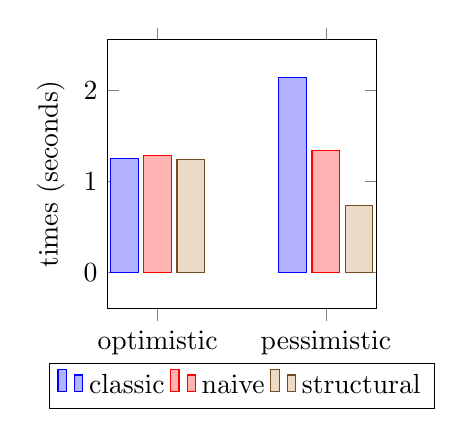
\begin{tikzpicture}
\begin{axis}[
    ybar, ymax = 2, ymin = 0.15,
    enlargelimits=0.3,
    width=5cm, height=5cm,
    legend style={at={(0.5,-0.2)},
      anchor=north,legend columns=-1},
    ylabel={times (seconds)},
    symbolic x coords={optimistic, pessimistic},
    xtick=data
    ]
\addplot coordinates {(optimistic,1.254) (pessimistic,2.142)};
\addplot coordinates {(optimistic,1.282) (pessimistic,1.337)};
\addplot coordinates {(optimistic,1.236) (pessimistic,0.733)};
\legend{classic,naive,structural}
\end{axis}
\end{tikzpicture}
 \captionof{figure}{revers$^o$ forward evaluation \\ for a list with a length of 90}
  \label{fair:plot-reverso}
\end{minipage}%
\begin{minipage}{.5\textwidth}
  \centering
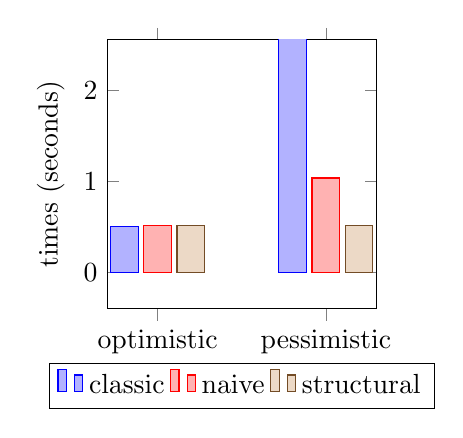
\begin{tikzpicture}
\begin{axis}[
    ybar, ymax = 2, ymin = 0.15,
    enlargelimits=0.3,
    width=5cm, height=5cm,
    legend style={at={(0.5,-0.2)},
      anchor=north,legend columns=-1},
    ylabel={times (seconds)},
    symbolic x coords={optimistic, pessimistic},
    xtick=data
    ]
\addplot coordinates {(optimistic,0.504) (pessimistic,300)};
\addplot coordinates {(optimistic,0.508) (pessimistic,1.035)};
\addplot coordinates {(optimistic,0.513) (pessimistic,0.513)};
\legend{classic,naive,structural}
\end{axis}
\end{tikzpicture}
 \captionof{figure}{sort$^o$ forward evaluation \\ for a list with a length of 5}
\label{fair:plot-sorto}
\end{minipage}
\end{figure*}

\begin{figure*}
\centering
\begin{minipage}{.5\textwidth}
  \centering
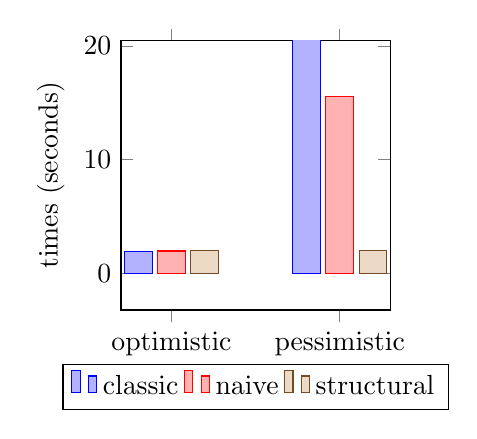
\begin{tikzpicture}
\begin{axis}[
    ybar, ymax = 16, ymin = 1.2,
    enlargelimits=0.3,
    width=5cm, height=5cm,
    legend style={at={(0.5,-0.2)},
      anchor=north,legend columns=-1},
    ylabel={times (seconds)},
    symbolic x coords={optimistic, pessimistic},
    xtick=data
    ]
\addplot coordinates {(optimistic,1.909) (pessimistic,300)};
\addplot coordinates {(optimistic,1.945) (pessimistic,15.516)};
\addplot coordinates {(optimistic,1.980) (pessimistic,1.978)};
\legend{classic,naive,structural}
\end{axis}
\end{tikzpicture}
 \captionof{figure}{``The Tower of Hanoi'' \\ solver evaluation}
\label{fair:plot-hanoi}
\end{minipage}%
\begin{minipage}{.5\textwidth}
  \centering
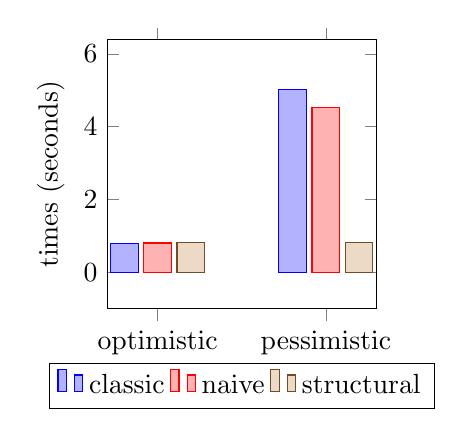
\begin{tikzpicture}
\begin{axis}[
    ybar, ymax = 5, ymin = 0.375,
    enlargelimits=0.3,
    width=5cm, height=5cm,
    legend style={at={(0.5,-0.2)},
      anchor=north,legend columns=-1},
    ylabel={times (seconds)},
    symbolic x coords={optimistic, pessimistic},
    xtick=data
    ]
\addplot coordinates {(optimistic,0.783) (pessimistic,5.019)};
\addplot coordinates {(optimistic,0.801) (pessimistic,4.522)};
\addplot coordinates {(optimistic,0.812) (pessimistic,0.817)};
\legend{classic,naive,structural}
\end{axis}
\end{tikzpicture}
 \captionof{figure}{``Bridge and torch problem'' \\ solver evaluation}
\label{fair:plot-bridge}
\end{minipage}
\end{figure*}

Now we will discuss evaluation. Целью эвалюации является выявления влияния порядка конъюнктов на эффективность трех различных семантик.

Первая семантика с предикатом $pred_{\mbox{\lstinline{true}}}$ близка к классическим реализациям \mk. В дальнейшем будем называть её {\bf left-biased}.

Вторая семантика с предикатом $pred_N$ соответсвует равномерному вычислению всех конъюнктов. Эту семантику будем назвать {\bf naive}.

Третья семантика с предикатом $pred_{\leq_{sr}}$ вычисляет структурно-рекурсивные конъюнкты, пока убывают структурно-рекурсивные аргументы. Её будем называть {\bf structural}.

For evaluation we've chosen two simple programs (list reversing and list sorting) and three more complicated (the ``Hanoi Towers''\footnote{\url{https://en.wikipedia.org/wiki/Tower_of_Hanoi}} solver, the
``Bridge and torch problem''\footnote{\url{https://en.wikipedia.org/wiki/Bridge_and_torch_problem}} solver and ``Water pouring puzzle''\footnote{\url{https://en.wikipedia.org/wiki/Water_pouring_puzzle}} solver).
% Для каждой программы мы сделали две версии. Оптимистичная версия --- это программа, в которой мы вручную подобрали оптимальный порядок конъюнктов и пессиместичная версия --- программа с неоптимальным порядком конъюнктов. В последующих диаграммах и таблице указаны средние значения 10 запусков тестов. Также для наивной равномерной конъюнкции мы подобрали количество разверток вручную. Для равномерной конъюнкции, основанной на структурной рекурсии, N было фиксировано и равно 100.
Each program was written in two versions: ``optimistic'' (with the order of important conjuncts set to provide the best performance) and ``pessimistic'' (with the order of important
conjuncts set to provide the worst performance). Also we evaluated list reversing and list sorting in both directions. In the case of the list reversing, queries \lstinline{(revers$^o$ [1;2;3] q)} and \lstinline{(revers$^o$ q [1;2;3])}\! will give the same answer \lstinline{q = [3;2;1]} but the ``optimistic'' order of conjuncts is different for them. In the case of list sorting, queries \lstinline{(sort$^o$ [1;2;3] q)} and \lstinline{(sort$^o$ q [1;2;3])} will give different answers. The first one gives sorted list \lstinline{q = [1;2;3]}, the second one gives all permutations of list \lstinline{[1;2;3]}\!\!. 

All benchmarks were run ten times, and the average time was taken. For the naive  semantics we cherry-picked the best value of unfolding bound manually. Structural arguments for each relations were detected automatically.

% На изображениях 12-15 представлены результаты апробации в виде столбцовых диаграмм. В оптимистичном случае результаты схожи для всех семантик. В пессиместичном случае время работы напрпавленной конъюнкции резко возрастает, время работы наивной равномерной конъюнкции также ворзрастает, но не так сильно. Равномерная конъюнкция, основанная на структурной рекурсии, демострирует схожую эффективность в сравнении с оптимистичным случаем.
Fig.~\ref{fair:plot-reverso}-\ref{fair:plot-bridge} show the results of evaluation in the form of bar charts. In the optimistic case, the results are similar for all semantics.
In the pessimistic case the evaluation time of the directed conjunction rapidly increases, the evaluation time of the naive fair conjunction also increases, but not so much.
The fair semantics based on structural recursion demonstrates a similar efficiency as in the optimistic case.

\begin{figure*} %[h!]
  \small
  \centering
  \begin{tabular}{ c | c | c | c | c | c | c | c }
    \multirow{2}{*}{relation} & \multirow{2}{*}{size} & 
    \multicolumn{2}{c}{left-biased semantics} &
    \multicolumn{2}{c}{naive semantics} &
    \multicolumn{2}{c}{structural semantics} \\
    \cline{3-8}
    & & optimistic & pessimistic & optimistic & pessimistic & optimistic & pessimistic  \\ 
    \hline
    \multirow{3}{*}{\begin{tabular}{c} forward \\ revers$^o$ \end{tabular}}
                 & 30   & 0.527 & 0.587  & 0.532 & 0.595   & 0.539 & 0.532 \\
                 & 60   & 0.639 & 0.947  & 0.643 & 0.790   & 0.657 & 0.577 \\
                 & 90   & 1.254 & 2.142  & 1.282 & 1.337   & 1.236 & 0.733 \\
    \hline
    \multirow{3}{*}{\begin{tabular}{c} backward \\ revers$^o$ \end{tabular}}
                 & 30   & 0.531 & 0.579  & 0.547 & 0.570  & 0.553 & 0.563 \\
                 & 60   & 0.655 & 0.875  & 0.667 & 0.812  & 0.668 & 0.681 \\
                 & 90   & 1.316 & 1.813  & 1.327 & 1.503  & 1.360 & 1.359 \\
    \hline
    \multirow{5}{*}{\begin{tabular}{c} forward \\ sort$^o$ \end{tabular}}
                 & 3    & 0.467 & 0.503  & 0.474 & 0.481  & 0.472 & 0.479 \\
                 & 4    & 0.484 & 4.679  & 0.485 & 0.493  & 0.490 & 0.488 \\
                 & 5    & 0.504 & $>$300 & 0.508 & 1.035  & 0.513 & 0.513 \\
                 & 6    & 0.526 & $>$300 & 0.237 & 14.369 & 0.544 & 0.547 \\
                 & 30   & 1.915 & $>$300 & 1.936 & $>$300 & 1.983 & 1.987 \\
    \hline
    \multirow{4}{*}{\begin{tabular}{c} backward \\ sort$^o$ \end{tabular}}
                 & 3    & 0.518 &  0.519 & 0.518 & 0.521  & 0.520 & 0.521 \\
                 & 4    & 0.533 &  0.856 & 0.534 & 0.540  & 0.534 & 0.537 \\
                 & 5    & 0.680 & 93.914 & 0.713 & 1.528  & 0.718 & 0.714 \\
                 & 6    & 2.931 & $>$300 & 2.947 & 59.647 & 2.938 & 2.936 \\
    \hline
    hanoi$^o$    & -    & 1.909 & $>$300 & 1.945 & 15.516 & 1.980 & 1.978 \\
    \hline
    bridge$^o$   & -    & 0.783 & 5.019  & 0.801 & 4.522  & 0.812 & 0.817 \\
    \hline
    water$^o$    & -    & 3.513 & $>$300 & 3.518 & $>$300 & 3.538 & 3.771

  \end{tabular}
  \caption{The results of evaluation: running times of benchmarks in seconds}
  \label{fair:evaluation-table}
\end{figure*}

% Более подробно результаты представлены на изображении 16. Можно заметить, что время работы программы sorto в пессиместичном случае очень быстро растет с увеличением длины списка для направленной конъюнкции и наивной равномерной. В случае с равномерной конъюнкцией, основанной на структурной рекурсии, пессиместичный случай растет сопостовимо с оптимистичным.
The results are presented in more detail in Fig.~\ref{fair:evaluation-table}. ``Hanoi Towers'' solver has name \lstinline{hanoi$^o$}, ``Bridge and torch problem'' solver has name \lstinline{bridge$^o$} and ``Water pouring puzzle'' solver has name \lstinline{water$^o$}. We can conclude that forward and backward \lstinline{sort$^o$} runtime in the pessimistic case increases very rapidly with increasing the list length for left-biased and naive fair semantics. In the case of the fair semantics based on structural recursion the running time in pessimistic case increases on a par with that in the optimistic one. Also the solver \lstinline{water$^o$} very slow in the pessimistic case for left-biased and naive fair. However, fair conjunction based on structural recursion pessimistic case is no different from an optimistic case.


% Подводя итог, равномерная конъюнкция, основанная на структурной рекурсии сопоставима по эффективности с направленной конъюнкцией. Более того, это конъюнкция слабо зависит от порядка конъюнктов.
To summarize, the fair semantics based on structural recursion does not introduce any essential overhead in comparison with left-biased semantics in an optimistic case. At the same time it
weakly depends on the order of the conjuncts, and thus demonstrates much better performance in the pessimistic case.

\section{Conclusion}
\label{conclusion}

We presented an approach for converting typed functional programs into relations. Relational conversion 
in many cases allows us to avoid tedious recoding of functional specifications into relational form and to 
concentrate on writing relational specifications only when their reconstruction from functions is impossible or 
undesirable. Our implementation works for the subset of OCaml; we evaluated it for a number of interesting 
examples and acquired some new relational solutions.

There is a number of directions for future research. First, a performance evaluation is desirable~--- at
present time we do not know, what slowdown factor is. Another problem is a development of an approach to
prove complete correctness (or refute this claim).


\bibliographystyle{ACM-Reference-Format}
\bibliography{main}

\end{document}
